% Z~toho plyne otázka, jaká funkcionalita je potřebná v~základním zařízení?
% Asi žádný systém, se kterým hráč přímo interaguje, není nutný v~každé hře.
% Jde tedy o~to vybrat takové systémy, které svými nároky nepřevýší užitečnost při hrách.
% Ze zkušeností považujeme za nejzákladnější systém nějaký světelný výstup, ten dokáže většinu her velmi příjemně ozvláštnit.
% Většinou je nezbytný i~uživatelský vstup, na což většinou stačí obyčejná tlačítka.
% Problém je ale určit jaké a~kolik jich bude potřeba.
% Některé hry vyžadují třeba jen jedno, ale takové, aby se do něj dalo co nejpohodlněji praštit v~běhu, protože je zrovna cílem ke stanovišti co nejrychleji doběhnout.
% Jiná hra může vyžadovat tlačítek víc, ale už není potřeba, aby byly tak velké, protože hráč při jejich používání nebude tak akční, ale bude třeba zadávat výsledek logického úkolu.
% Univerzálnější je tedy nepoužívat tlačítka, ale nějaký systém, který se dá softwarově přizpůsobit.
% Příkladem může být dotyková plocha, která se dá softwarově rozdělit na různé oblasti sloužící jako tlačítka a~i~během hry se tak dá počet tlačítek měnit.
% Další důležitou vlastností je možnost komunikace s~ostatními zařízeními, která do hry přináší novou možnost jak stanoviště propojit a~také pohodlnou metodu jak stanoviště nastavit přes telefon.
% V~neposlední řadě je potřeba zvukový výstup, který může být použit např. jako potvrzení zadaného hesla.

% Z~toho nám tedy plyne diagram \ref{fig:diagram_zanoreni_0}.
% \begin{figure}[h]
%     \centering
%     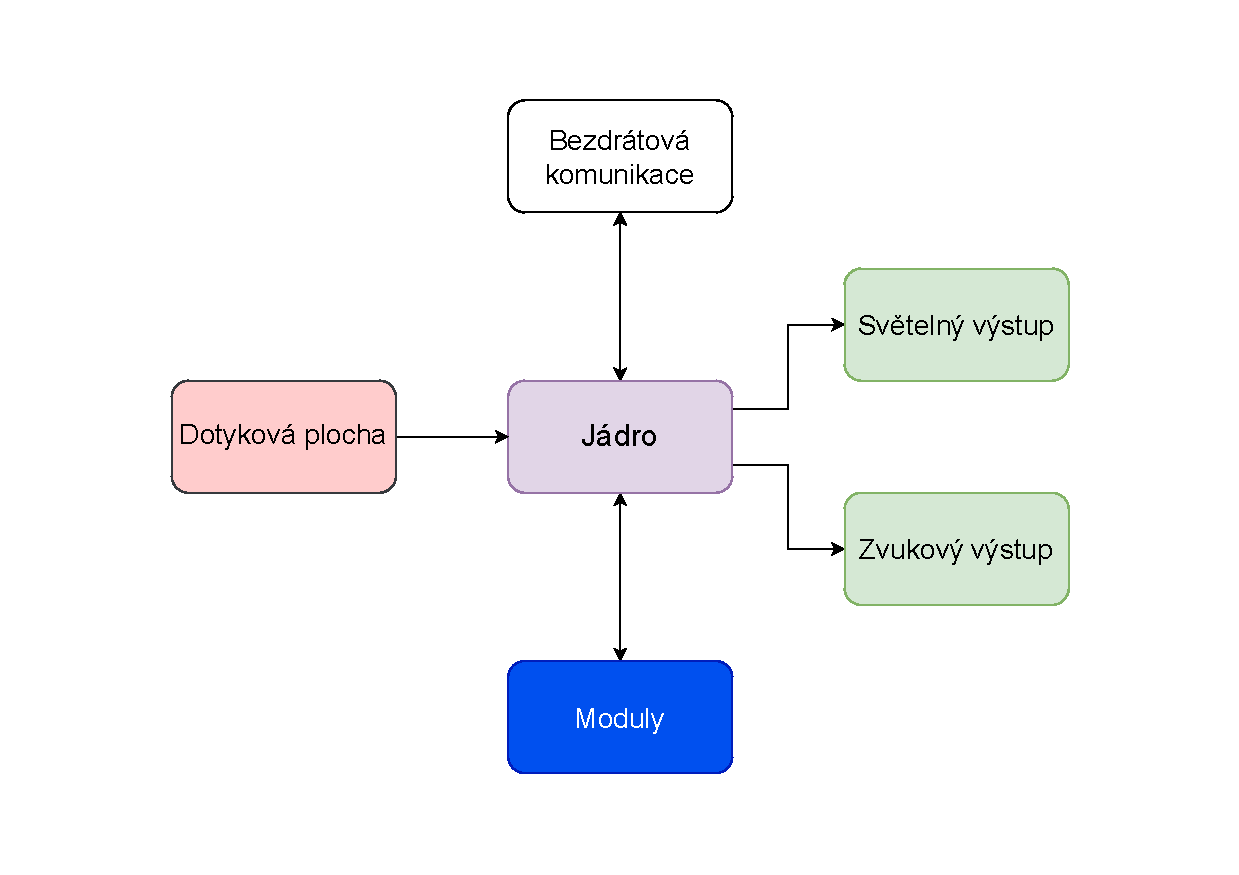
\includegraphics[width=0.65\textwidth]{text/TeoretickyUvod/AplikaceHernichZarizeni/diagram/zanoreni_0.pdf}
%     \caption{Úvodní blokové schéma zařízení}
%     \label{fig:diagram_zanoreni_0}
% \end{figure}

% \newpage

Co se~světelného výstupu týče, na~signalizaci různých stavů je~vhodné používat různé barvy světel.
% Jaký vzhled by~ale měl mít zdroj barevného světla na~podobném zařízení?
Jak je~uvedeno výše, není potřebné suplovat grafický display, za~tímto účelem se~dá použít propojení s~telefonem.
Informace, kterou by~zařízení mohlo často poskytovat je~čas a~směr, např. čas do~konce kola nebo směr k~dalšímu úkolu.
Podobné informace se~dají elegantně zobrazit na~kruhu.
Protože má~být stanoviště viditelné i~z~větší vzdálenosti, je~tedy otázkou, zda použít jen jeden kruh, tak aby byl dostatečně viditelný, nebo jich použít více. %%TODO: otázka co~s~totu otázkou?
Zobrazování pracuje ve~dvou režimech, čtení na~dálku a~čtení na~blízko.
Pro čtení na~blízko je~cílem přímá interakce se~zařízením např. už~zmiňované zadávání hesla.
Čtení na~dálku je~naopak určeno pro předávání informací hráči, když právě přímo neinteraguje se~stanovištěm, např. který tým má~zrovna povolený přístup.
Proto je~vhodné mít kruhů více, aby bylo možné zobrazovat tyto informace na~různých kruzích, které mohou navíc být svému účelu přizpůsobeny.
Jeden kruh tak může svítit jen jedním směrem, aby ho~hráč viděl celý najednou pro blízkou interakci, zatímco druhý kruh může svítit do~všech stran, aby byl vidět z~co~nejvíce míst.

Potřeba propojení s~telefonem nám omezuje možnosti co~se týče bezdrátové komunikace, protože telefony jsou většinou vybaveny Bluetooth a~WiFi.
Také se~v~telefonech rozšiřuje NFC, to~je však pro tuto aplikaci z~důvodu krátkého dosahu nevhodné.

Posledním systémem, který je~potřeba, je~zvukový výstup.
Protože většinou stačí jen jednoduchá zvuková odezva, není potřeba plnohodnotný zvukový systém.
Pro hry, které budou potřebovat přehrávat nějakou nahrávku, bude samostatný zvukový modul, případně je~možnost nahrávku přehrát přes uživatelův telefon.
V~základním zařízení je~proto potřeba jen jednoduchý bzučák, například jako odezva na~kliknutí.

Můžeme tedy diagram upravit na~\ref{fig:diagram_zanoreni_1}.
\begin{figure}[h]
    \centering
    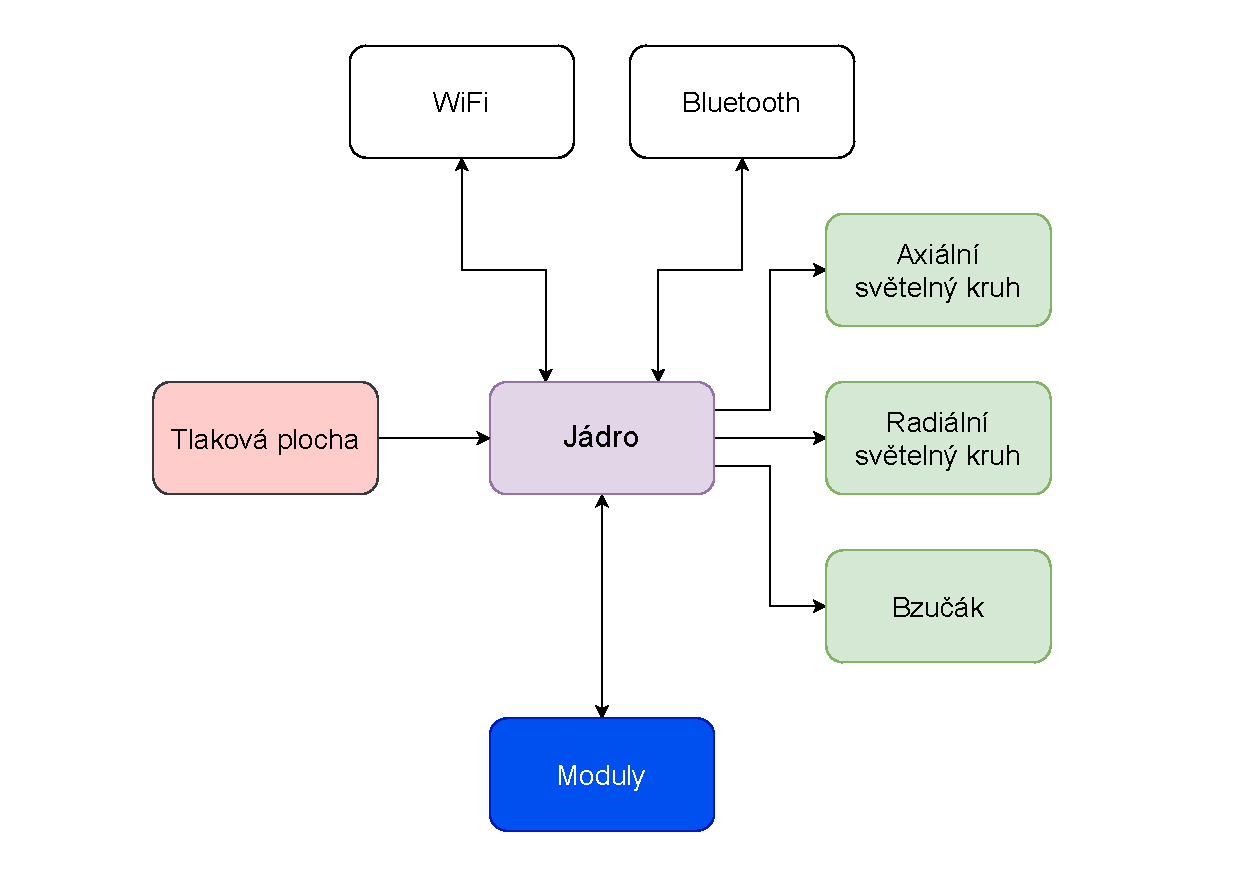
\includegraphics[width=0.65\textwidth]{text/TeoretickyUvod/AplikaceHernichZarizeni/diagram/zanoreni_1.pdf}
    \caption{Základní blokové schéma zařízení}
    \label{fig:diagram_zanoreni_1}
\end{figure}

Celé zařízení by~také mělo být alespoň částečně voděodolné, aby se~dalo použít třeba i~za~deště.

\vspace{-10mm}